%%
%% This is file `example_DarkConsole.tex',
%% generated with the docstrip utility.
%%
%% The original source files were:
%%
%% examples_kmbeamer.dtx  (with options: `DarkConsole')
%% Copyright (c) 2011-2013 Kazuki Maeda <kmaeda@users.sourceforge.jp>
%% 
%% Distributable under the MIT License:
%% http://www.opensource.org/licenses/mit-license.php
%% 

%%% もし pdfTeX や LuaTeX を使うなら dvipdfmx オプションを外す.
% \documentclass[dvipdfmx]{beamer}

% Modified by LianTze Lim to work with fontspec/xelatex
\documentclass{beamer}
\usepackage[ngerman]{babel}
\usepackage{mathspec}
\usepackage{xeCJK}
\setCJKmainfont{IPAPMincho}
\setCJKsansfont{IPAGothic}
\setCJKmonofont{IPAGothic}

% You can set fonts for Latin script here
\setmainfont{FreeSerif}
\setsansfont{FreeSans}
\setmonofont{Latin Modern Mono}

\usetheme{DarkConsole}

%%%%%%%%%%%%%%%%%%%%%%%%%%%%%%%%%%%%%%%%%%%%%%%%%%%%%%%%%%%%%%%%%
% Neue Sachen::
%%%%%%%%%%%%%%%%%%%%%%%%%%%%%%%%%%%%%%%%%%%%%%%%%%%%%%%%%%%%%%%%%
%\addtobeamertemplate{frametitle}{
%   \let\insertframetitle\insertsectionhead}{}
%\addtobeamertemplate{frametitle}{
%   \let\insertframesubtitle\insertsubsectionhead}{}
%
%
%\makeatletter
%  \CheckCommand*\beamer@checkframetitle{\@ifnextchar\bgroup\beamer@inlineframetitle{}}
%  \renewcommand*\beamer@checkframetitle{\global\let\beamer@frametitle\relax\@ifnextchar\bgroup\beamer@inlineframetitle{}}
%\makeatother
\usepackage{graphicx}
\usepackage{array}
%%%%%%%%%%%%%%%%%%%%%%%%%%%%%%%%%%%%%%%%%%%%%%%%%%%%%%%%%%%%%%%%%
% Ende neue Sachen
%%%%%%%%%%%%%%%%%%%%%%%%%%%%%%%%%%%%%%%%%%%%%%%%%%%%%%%%%%%%%%%%%

%% \AtBeginDvi{\special{pdf:tounicode EUC-UCS2}} % EUC の場合
%% \AtBeginDvi{\special{pdf:tounicode 90ms-RKSJ-UCS2}} % SJIS の場合

%%% もし LuaTeX で日本語を出力するなら以下をコメントアウト.
%% \usefonttheme{luatexja}
%% \hypersetup{unicode}

%%% 日本語を使うなら以下を入れると定理環境中のフォントが立体になる.
%%% 欧文なら不要.
%%% LLT: Comment out this line if your presentation is in English or other European languages
\setbeamertemplate{theorems}[normal font]

\title{Projektpraktikum I}
\subtitle{Serie 4, Teil 1}
\author{Arsen Hnatiuk, Max Huneshagen}

\begin{document}

\begin{frame}
  \maketitle
\end{frame}

\begin{frame}{Inhalt}
  \tableofcontents
\end{frame}

\section{Methode der kleinsten Quadrate}

\begin{frame}{Herleitung}
  Sei $A\in \mathbb{R}^{n\times m}$,  $b\in \mathbb{R}^n$ mit $n>m$.\\
  \begin{itemize}
  \item Ziel: \glqq Lösen\grqq ~des überbestimmten Gleichungssystems 
  \begin{align}
  Ax=b
  \end{align}
  durch Finden des Minimums
  \begin{align}
  \min\limits_{x\in\mathbb{R}^m}\|Ax-b\|_\infty.
  \end{align}
\item Vorgehen:
\begin{itemize}
\item Finden der Q-R-Zerlegung:
\begin{align}
A=QR, \text{~~~}Q\in  O(n), R\in \mathbb{R}^{n\times m}\text{ obere Dreiecksmatrix}
\end{align}
\item mit $z:=Q^Tb=:
\begin{pmatrix}
z_1\\
\hline
z_2
\end{pmatrix}$ und $R=:\begin{pmatrix}
R_1\\
0
\end{pmatrix}$, wobei $z_1\in\mathbb{R}^{m}$ und $R_1\in\mathbb{R}^{m\times m}$ ergibt sich:
\begin{align}
R_1x=b\text{,~~~}  \min\limits_{x\in\mathbb{R}^m}\|Ax-b\|_\infty=\|z_2\|
\end{align}

\end{itemize}
  \end{itemize}
  



\end{frame}

\begin{frame}{Problemstellung [0]}
\begin{itemize}
\item Pegelstände an 3 verschiedenen Pegeln beobachtet:
\begin{align}
p, a_1, a_2 \in \mathbb{R}^m
\end{align}
\item 2 Ansätze:
\begin{itemize}
\item Einfache lineare Regression:
\begin{align}
p =b_0+b_1a_1
\label{eq:lin_reg}
\end{align}
\item Mehrfachregression:
\begin{align}
p =b_0+b_1a_1+b_2a_2
\label{eq:mehr_reg}
\end{align}
\end{itemize}
\item \eqref{eq:lin_reg} und \eqref{eq:mehr_reg} führen auf die folgenden Gleichungssysteme:
\end{itemize}

\end{frame}

\begin{frame}{Problemstellung [0]}
\begin{itemize}
\item \eqref{eq:lin_reg} und \eqref{eq:mehr_reg} führen auf die folgenden (überbestimmten) Gleichungssysteme:
\begin{itemize}
\item Lineare Regression:
\begin{align}
\begin{pmatrix}
1 & \vrule \\
\vdots & a_1\\
1 & \vrule
\end{pmatrix}
\begin{pmatrix}
b_0\\
b_1
\end{pmatrix}
=
\begin{pmatrix}
\vrule\\
p\\
\vrule
\end{pmatrix}
\end{align}
\item Mehrfachregression:
\begin{align}
\begin{pmatrix}
1 & \vrule & \vrule\\
\vdots & a_1&a_2\\
1 & \vrule &\vrule
\end{pmatrix}
\begin{pmatrix}
b_0\\
b_1\\
b_2
\end{pmatrix}
=
\begin{pmatrix}
\vrule\\
p\\
\vrule
\end{pmatrix}
\end{align}
\end{itemize}
\item Lösung erfolgt über Methode der kleinsten Quadrate
\end{itemize}
\end{frame}

\section{Experimente}
\begin{frame}
Extrem hübsche Bilder usw.\\~\\
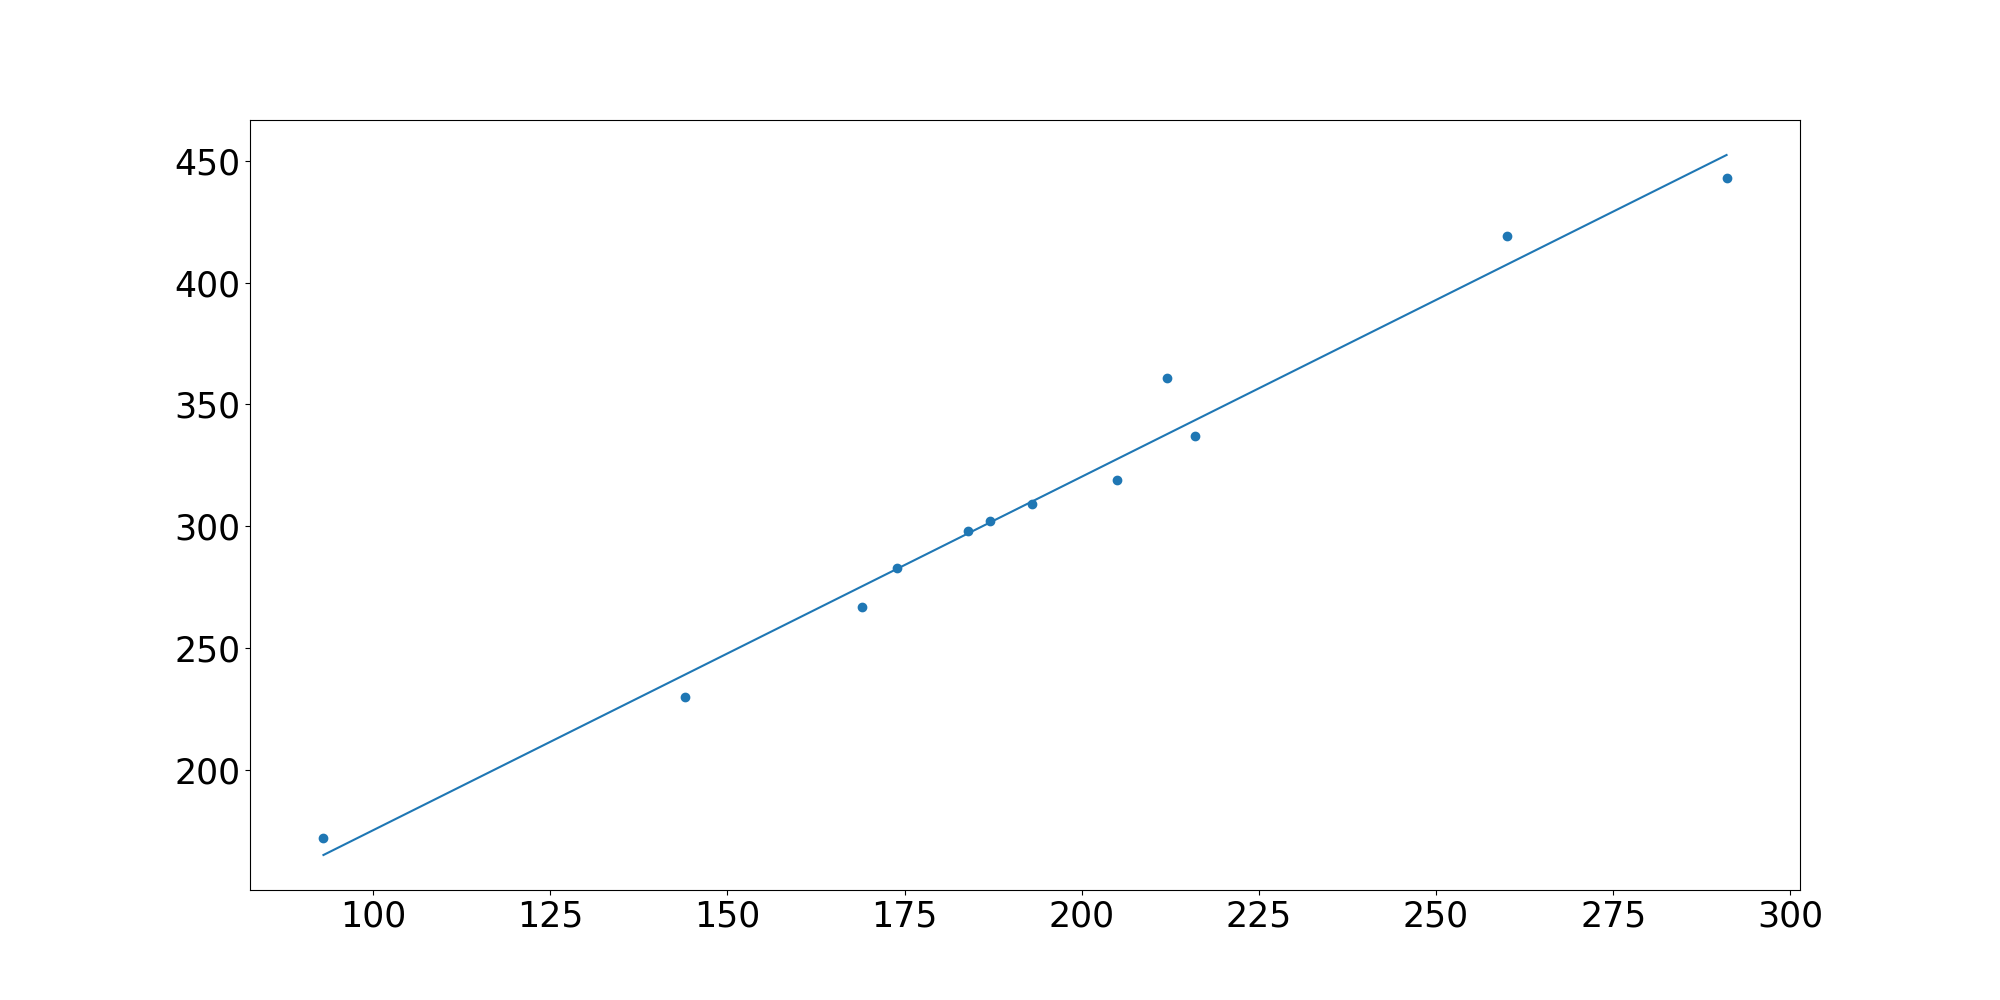
\includegraphics[width=\textwidth]{Beispielbild}
\end{frame}
\end{document}
\endinput
%%
%% End of file `example_DarkConsole.tex'.
